\chapter{Testing and configuring Snort}
\minitoc
\emph{As the installation of Snort, Sguil, Snorby has been completed, we will now focus on the testing and configuration of Snort.}

\section{Introduction}

In order to make sure that Snort is actually protecting our network against numerous and various anomalies, it is essential to test Snort against various attacks. Based on how Snort reacts on the attacks, we will configure Snort, that is, modifying the rules (signatures), add rules if no alerts are raised or removing some of the rules that are triggering false alerts. Not only can one adjust the rules, also thresholds and limitations of how many alerts each rule is allowed to generate can be set. \\ \\
Of course, false positives will also be generated and the art of configuring Snort is minimizing the amount of false positives and maximizing the generation of alerts of real threads.

The difficulty lies in the fact to distinguish real threads from false positives. One may also not forget that each network is different, so there does not exist an ``optimal'' or ``perfect'' configured set of rules for all networks. Each network has to be examined and configured independently. However, this process takes up some time. Speaking in terms of weeks or even months is not unusual.

\section{Testing environment}

To perform the actual tests, a correct working network is needed. All the attacks are performed in a designated testing lab.

How does this work? All computers are connected to the same switch. Security Onion is installed in VirtualBox on a physical machine. 

The management interface of Security Onion has the IP address of 192.168.1.3-8. Remember that we used DHCP for the management interface, this explains the range. Note that the sniffing interface has promiscious mode set and therefore does not have an IP address. \\ \\
The target (victim) computer has the IP address of 192.168.1.17 (static IP). All attacks are launched to this machine. \\ \\
The attacker (ourself) uses a computer with IP address 192.168.1.40 (static IP) will initiate various attacks on the network. \\ \\
\textbf{Summary}
\begin{itemize}
\item Victim host
	\begin{itemize}
	\item OS: Windows 7 Professional SP1 64 bit
	\item IP address: 192.168.1.17
	\end{itemize}
\item Attacking host
	\begin{itemize}
	\item OS: Windows 7 Professional SP1 32 bit
	\item IP address: 192.168.1.40
	\end{itemize}
\item Security Onion (Snort)
	\begin{itemize}
	\item OS: Xubuntu 12.04 LTS 64 bit
	\item IP address (eth0): 192.168.1.3-8
	\item IP address (eth1): none - promiscious mode
	\end{itemize}
\end{itemize}

\section{What types of attacks will be performed?}

Various types of network and host attacks will be executed on the network in order to test Snort's reaction. These types include:
\begin{itemize}
\item Port scans
	\begin{itemize}
	\item Basic port scan
	\item Advanced port scan
	\end{itemize}
\item Webserver attacks
	\begin{itemize}
	\item VISA card numbers sent in plain text over the network
	\item XSS
	\item SQL Injection
	\item Command Injection
	\end{itemize}
\item FTP server attacks
	\begin{itemize}
	\item FTP root access
	\item FTP malicious payloads
	\item Various other FTP attacks
	\end{itemize}
\item SSH attacks
\item SMB attacks
	\begin{itemize}
	\item List shares
	\item List users
	\item Login attempts
	\item Bruteforce attempts
	\end{itemize}
\item Database attacks
	\begin{itemize}
	\item Database scanning
	\item Login attempts (including root access)
	\item Bruteforce attempts
	\end{itemize}
\item Trojan and virus injection / infection
\item DOS attacks
\end{itemize}

\subsection{Motivation for the choice of the attacks}

Why were these nine types of attacks chosen? The attacks are based on the actual services provided by some servers in my own home network. I have for example a web server running, an FTP server, a Samba server and a MySQL server. All those servers are running on Linux and to remotely login on those servers, SSH is frequently used.

So that is why webserver, FTP and SMB attacks will be performed. In addition, each hacker starts by scanning the network for running computers and once a computer has been found, a port scan is executed to scan the host for open ports which the hacker can exploit.

\section{Testing methods}

On the victim host, a webserver, FTP server, Samba server, database server and SSH server are installed. The correct functioning of those services is controlled and when it is confirmed that the service / server that is about to be attacked functioning properly, the actual attack is performed.

After the attack has been performed, Sguil is checked for realtime events. Remember that Snort writes its ``findings'' to the Sguil database. When the attack is listed, it means that Snort has successfully picked up / recognized the attack

Obviously, all of the above attacks can also be performed in my real network, but especially for the DOS attack and the Trojan infections, I chose not to use my real network and to set up a private, testing network.

\section{First things first: basic configuration of Snort}

First of all, we need to verify the network settings. Therefore, the ``ifconfig'' command is run. In addition, we also have a look at ``/etc/network/interfaces'' to confirm the settings.

\begin{figure}[h]
    \centering
    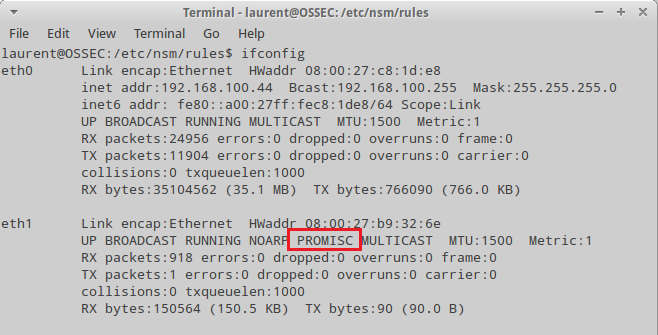
\includegraphics[width=0.85\textwidth]{VM_Network.png}
    \caption{Network settings are correct. eth0, the management interface received an IP address from the DHCP server. eth1 runs in promiscious mode and captures all the packets on the network. No IP address has been set (as it should be).}
\end{figure}

\begin{figure}[h]
    \centering
    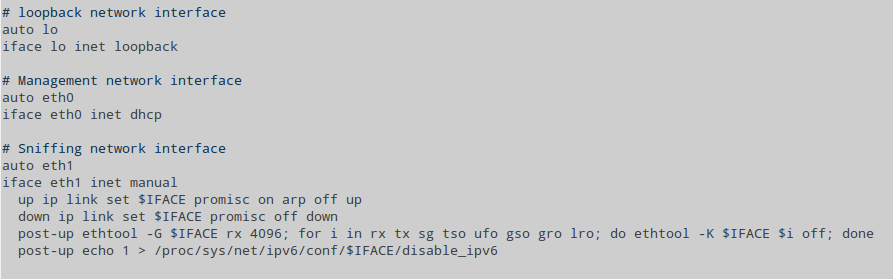
\includegraphics[width=0.85\textwidth]{VM_network_3.png}
    \caption{Confirmation of the network settings.}
\end{figure}

After having verified that the network settings are correct, we can configure some of the basic options of Snort. This includes network settings and is performed in ``snort.conf''. For example, the network segments on which Snort has to listen have to be configured.
\clearpage
\begin{figure}[h]
    \centering
    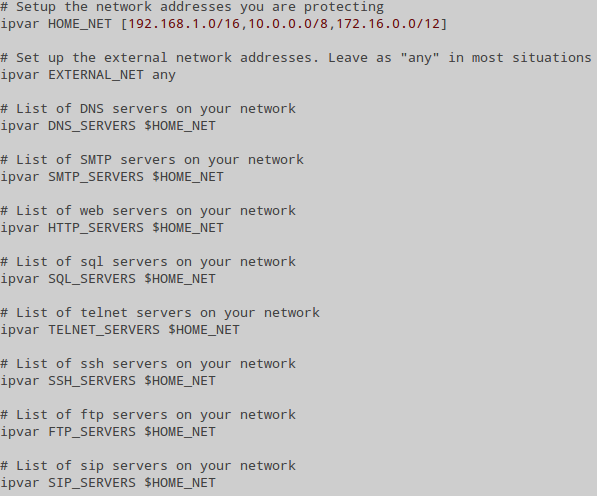
\includegraphics[width=0.85\textwidth]{VM_Network_2.png}
    \caption{We are working on the 192.168.1.0/24 network, but by means of testing, we have setup Snort to listen on the /16 subnet (255.255.0.0). As it will turn out, this will \textbf{not} affect the correct working of Snort. So one could randomly choose a value (8,16 or 24).}
\end{figure}

\newpage

\subsection{Configuring Snort rules}

Throughout this paper, we will frequently modify and add Snort rules (signatures), so an explanation of how a Snort rule is composed is given first. \\ \\
Most Snort rules are written in a single line. When a rules needs to span multiple lines, this can always be performed by adding a backslash ($\backslash$) at the end of the line.

Snort rules consist of two main parts: the rule header and multiple rule options. The header contains the rule's action method, protocol, source IP, source port, destination IP and destination port.

The rule options contains alert messages, signature ids, revisions and many more options. \\ \\
Below is the general layout of a Snort rule. \\ \\
\textbf{action protocol sourceIP sourcePort $->$ destinationIP destinationPort (OPTIONS);} \\ \\
To clear things up, an example is provided. \\
Consider following rule:

\textbf{alert icmp any any $->$ any any (msg:``ICMP ping"; sid:100002;)} \\ \\
This could be read as follows: ``alert all ICMP traffic from any source IP, from any port to any destination IP and to any destination port. Alert as ``ICMP ping'' and the unique id of the rule is 100002.''. \\ \\
Action can be one the following \citep{SnortRules}:
\begin{itemize}
\item alert: an alert is generated after which the packet is logged.
\item log: just log the packet, do not generate any alerts.
\item pass: ignore the packet.
\item drop: log and block the packet.
\item reject: log and block the packet and sent a TCP reset or ICMP port unreachable when TCP or UDP is used, respectively.
\end{itemize}
Protocol can be one the following \citep{SnortRules}:
\begin{itemize}
\item TCP
\item UDP
\item ICMP
\item IP
\end{itemize}
The IP address can be an ordinary IP address or an address/CIDR combination. For example, 192.168.100.0/24 would mean the block of addresses from 192.168.100.1 till 192.168.100.254.

\newpage

\subsection{Updating the rules using PulledPork}

After installing Snort (Security Onion), it is a good practise to update the ruleset, just as one may do when one has just installed an antivirus program. This is done using the ``update-rules'' command.

One could make a cron-job of this command to run it, for example, every day at 3 am.

\begin{figure}[h]
    \centering
    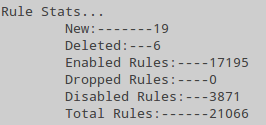
\includegraphics{VM_Pulledport_rules.png}
    \caption{After PulledPort has run, one can notice that 19 new rules have been downloaded and added to the ruleset of Snort.}
\end{figure}

\section{Confirming that Snort is actually working}

To confirm that all the agents (sensors) and the servers are running, the following command is executed: ``sostat -quick''. Which yields following output:

\begin{figure}[h]
    \centering
    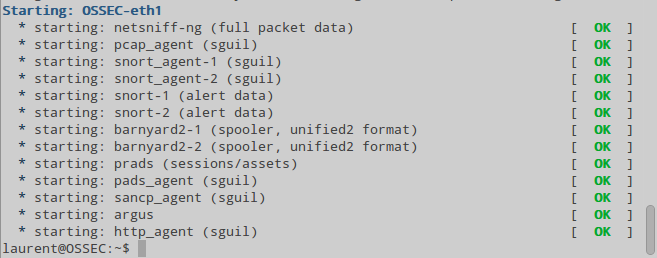
\includegraphics{VM_OK.png}
    \caption{Everything is running fine.}
\end{figure}


However, we cannot assume that, just by installing and configuring Snort - where everything \textbf{seems} to be working, that everything \textbf{is} actually working. To convince myself, a simple Snort rule has been made to detect and alert for any ICMP Ping traffic on the network: \\

\textbf{alert icmp any any $->$ any any (msg:``ICMP"; sid:100002;)} \\ \\
When pinging from the attack machine to the victim, Snort indeed picks up the ICMP traffic and fires a corresponding alert, as well as storing the information in the database. This can be seen in the screenshot below.

\begin{figure}[htb]
    \centering
    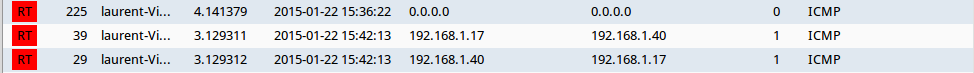
\includegraphics[width=0.95\textwidth]{VM_ICMP.png}
    \caption{Ping traffic gets picked up by Snort.}
\end{figure}

Notice that this rule can also be used to detect ping traffic from a network scanner which is used to detect how many hosts are online and what their IP address is.

\section{The actual penetration testing / attacks}

\subsection{Port scans}

Once the attacker knows which hosts are online, he can start querying a host to determine what services are running on the host or what types of protocols the host supports. This is the first phase in a network attack: the reconnaissance phase. 

\subsubsection{Unfragmented packets}

Nmap is used to execute the portscan. The exact command executed is \\
\textbf{nmap -T4 -A -v 192.168.100.17}. \\ \\
How did Snort react on this? It detected successfully the querying of multiple open ports, as one can see in the following screenshot. Therefore, no additional rules or extra configuration are necessary.

\begin{figure}[h]
    \centering
    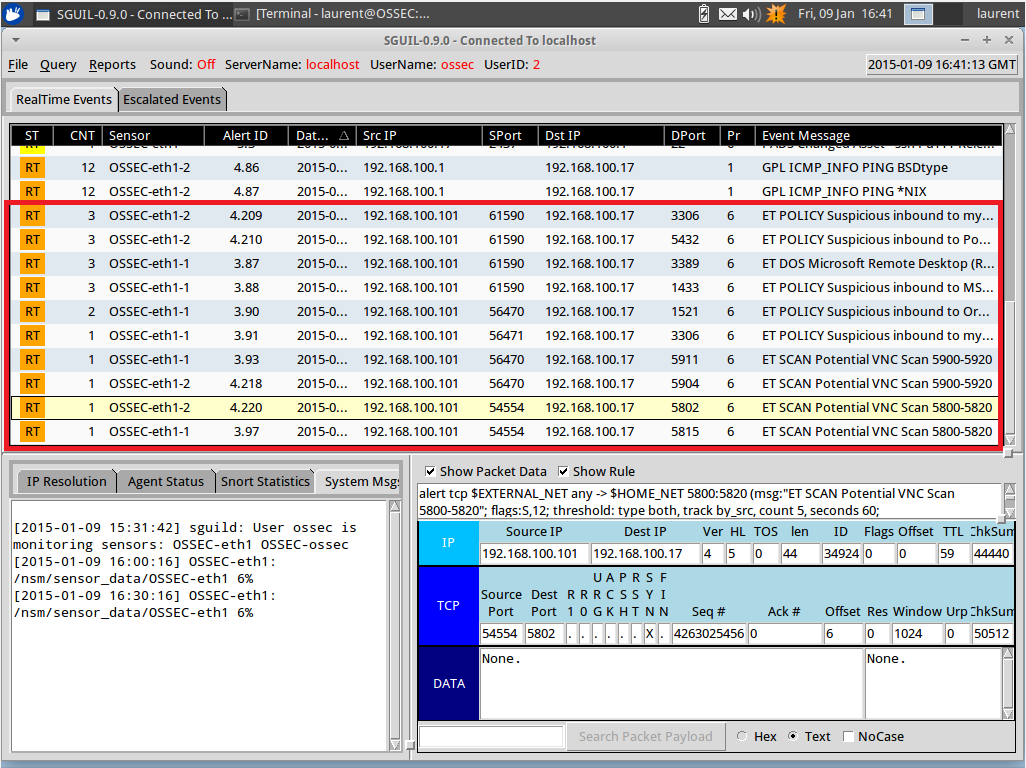
\includegraphics[width=0.85\textwidth]{VM_portscan_2.png}
    \caption{Unfragmented port scanning gets picked up by Snort.}
\end{figure}
\clearpage
\subsubsection{Fragmented SYN packets}

But what if the packets are fragmented into tiny little IP fragments? This way, an attacker hopes to evade packet filters.

Let us test this by executing a fragmented SYN scan:\\
\textbf{nmap -T4 -A -Ss -f -v 192.168.100.17} \\ \\
Unfortunately, Snort did NOT pick up on this. It was unable to recognize the executed port scan. So this means that additional rules have to be added to increase it's detectability.
Thus following rules were added:
\begin{figure}[h]
    \centering
    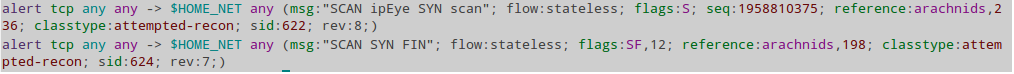
\includegraphics[width=0.95\textwidth]{VM_SynNull_3.png}
    \caption{Rules to detect SYN port scans}
\end{figure}
Then the same command was executed again, but still Snort didn't detect the fragmented SYN packets. \\
But maybe we could enable some preprocessors to enhance / extent Snort's ability to detect more threads? In this case, the ``frag3'' preprocessor seems like the ideal choice. Let us enable it.
\begin{figure}[h]
    \centering
    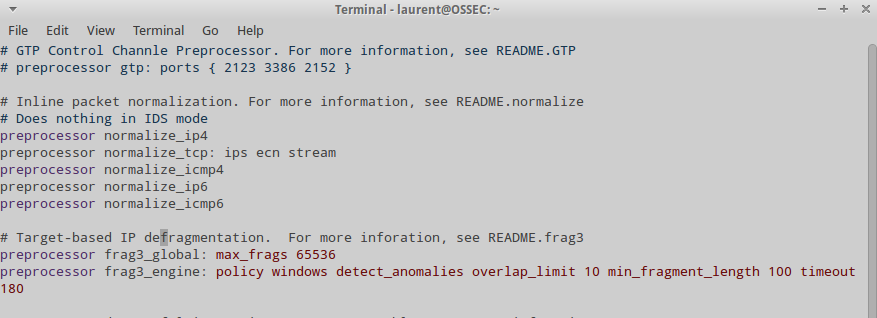
\includegraphics[width=0.85\textwidth]{VM_frag.png}
    \caption{Frag3 preprocessor enabled}
\end{figure}
Then once again, the same nmap command it executed, but Snort would STILL NOT pick up any fragmented SYN packets.

\subsubsection{NULL and XMAS scans}

First, note that SYN, NULL and XMAS are flags that are set in the TCP header. The idea behind these NULL and XMAS scans is that most IDSs look out for SYN packets, but a closed port should respond with an RST when receiving packets, whereas an open port would just drop them, because it is listening for SYN packets. This way, a connection is never made and thus a SYN packet is never sent. And thus the port scan remains hidden.

Let us find out how Snort reacts on NULL and XMAS scans. Therefore, following nmap command is executed: \\ \\
\textbf{nmap -T4 -A -sN -sX -v 192.168.100.17}. \\ \\
Not surprisingly, the port scans are NOT detected. Thus it is time to add some rules.

\begin{figure}[h]
    \centering
    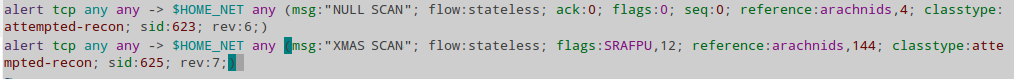
\includegraphics[width=0.95\textwidth]{VM_XMAS_2.png}
    \caption{Rules to detect NULL and XMAS port scans}
\end{figure}

After adding the rules, saving the file and restarting Snort by executing the ``sudo rule-update'' command, the same nmap command is executed again. This time Snort indeed does pick up the port scans as one can see in the following screenshot.

\begin{figure}[h]
    \centering
    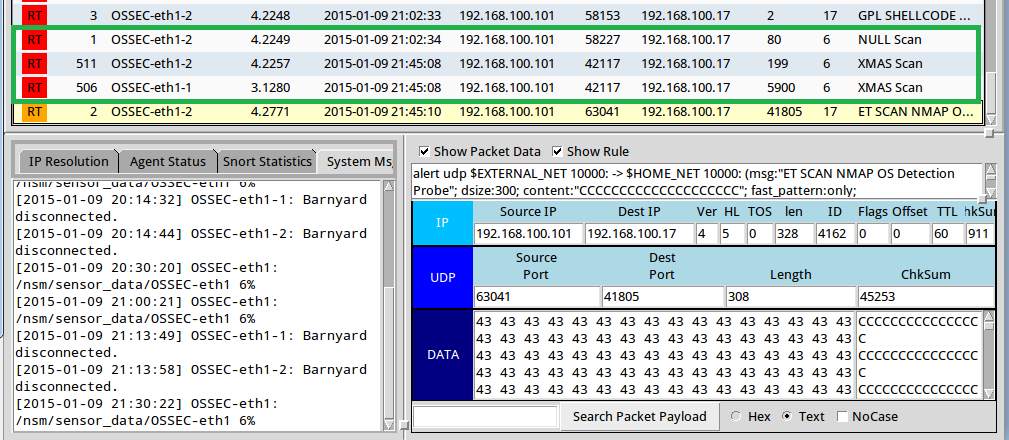
\includegraphics[width=0.95\textwidth]{VM_XMAS.png}
    \caption{This time, NULL and XMAS scans are detected}
\end{figure}

\clearpage

\subsection{Webserver attacks}

I setup a small webserver in the testing environment in order to perform some webserver attacks. The webserver runs on Apache2. 

\subsubsection{Testing for web traffic}

Before proceeding with the next type of attack, the HTTP webserver attacks, we first want to make sure that Snort picks up any HTTP traffic. Therefore, the following rules has been created: \\

\textbf{alert tcp any any $->$ any 80 (msg:"HTTP Traffic"; sid:100003;)} \\

\begin{figure}[h]
    \centering
    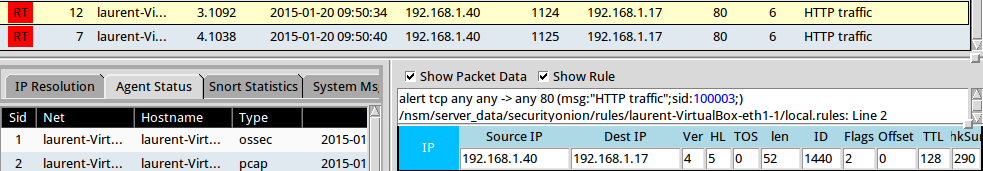
\includegraphics[width=0.85\textwidth]{VM_HTTP_1.png}
    \caption{Snort sees the HTTP traffic and alerts for it.}
\end{figure}

As one can observe, Snort successfully picks up any HTTP Traffic.

\subsubsection{VISA Card numbers sent in plain text}

Snort can also be used to detect sensitive information in clear text that circulates around the network (i.e., when a VISA Card number is sent in plain text in a HTTP Post). This way, an attacker that is sniffing the network can intercept those numbers.

The VISA Card number is 16 digits long and starts with a ``4''. For example, the number ``4000444062010002'' is a valid VISA Card number. \\

First, a regular expression has to be made to detect the format of a VISA Card number. Consider following expression: \\
\textbf{4$\backslash$ d\{3\}($\backslash$ s$|$-)?$\backslash$ d\{4\}($\backslash$ s$|$-)?$\backslash$ d\{4\}($\backslash$ s$|$-)?$\backslash$ d\{4\}} \\
This would read as follows: Start with a 4, then any 3 digits, then a space or dash or nothing, then any 4 digits, then a space or a dash or nothing, then any 4 digits, then a space or a dash or nothing, then any 4 digits. \\ \\
Eventually, the final Snort rule looks like: 

\begin{figure}[h]
    \centering
    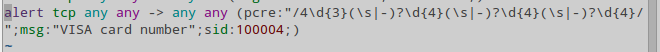
\includegraphics[width=0.85\textwidth]{VM_VISA.png}
    \caption{The Snort rule to detect plain text VISA numbers sent in plain text over the network.}
\end{figure}
\clearpage
The VISA Card number is filled in and the form is submitted\ldots.

\begin{figure}[h]
    \centering
    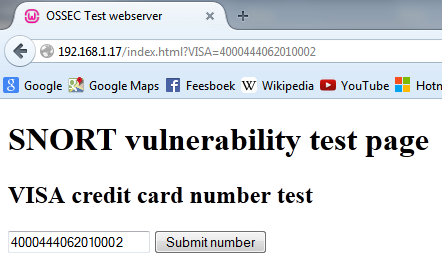
\includegraphics[width=0.85\textwidth]{VM_VISA_2.png}
    \caption{The VISA Card number entered in the textfield and the submission of the data in the textfield.}
\end{figure}

\ldots after which Snort triggers an alert.
\begin{figure}[h]
    \centering
    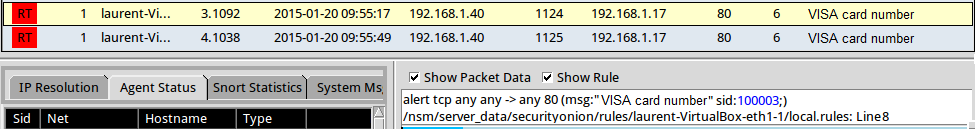
\includegraphics[width=0.85\textwidth]{VM_VISA_3.png}
    \caption{Snort alerts for the VISA Card numbers sent in plain text over the network.}
\end{figure}

\clearpage

\subsubsection{Cross-site scripting (XSS) attack}

Sometimes, one can abuse an URL of a webpage to inject JavaScript code into the page. This is called a cross-site scripting (XSS) vulnerability. If a hacker gives the modified URL to someone else and he can get this person to click on the modified links, a hacker / attacker can achieve the following: change the content of the page, steal cookie values, gain access to the user's history, \ldots. This is why we want to detect this. \\ \\
Therefore, I made a vulnerable PHP webpage myself, to exploit an XSS atack. The page takes the ``name'' parameter from the URL and displays it on the page. But this makes is ideal for an XSS attack.

\begin{figure}[h]
    \centering
    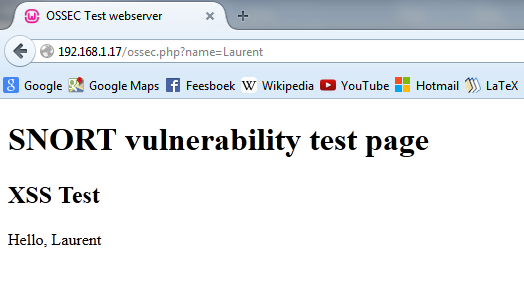
\includegraphics[width=0.85\textwidth]{VM_XSS_1.png}
    \caption{The vulnerable webpage before the attack. It displays the string value that is provided in the ``name'' parameter in the URL}
\end{figure}
Then, the following script is injected into the page: \\
\textbf{$<$script$>$alert('XSS vulnerability')$<$/script$>$}. \\
Which yields following output:

\begin{figure}[h]
    \centering
    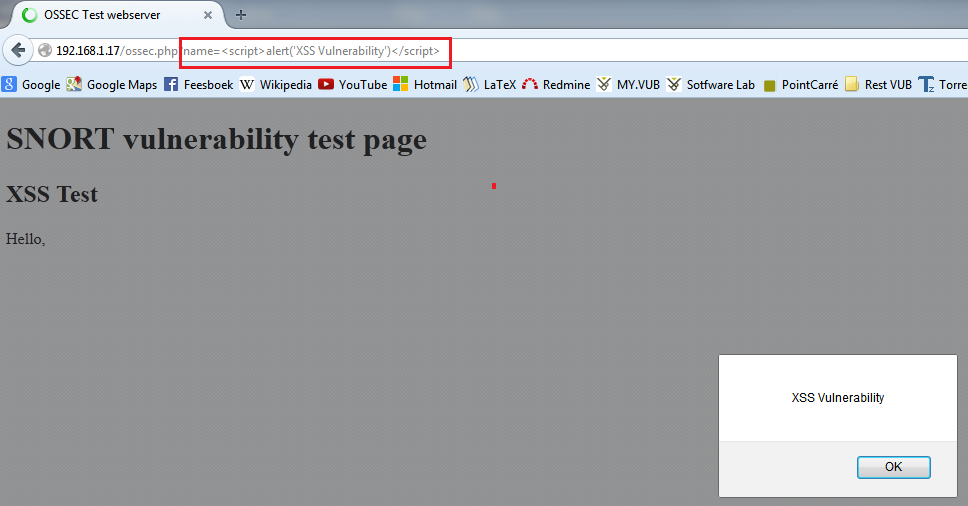
\includegraphics[width=0.75\textwidth]{VM_XSS_2.png}
    \caption{The script in action\ldots}
\end{figure}

As one can observe, the script is indeed successfully injected into the webpage.

\begin{figure}[h]
    \centering
    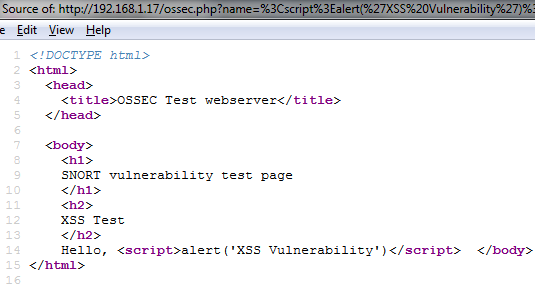
\includegraphics[width=0.85\textwidth]{VM_XSS_3.png}
    \caption{The script is successfully injected into the PHP page.}
\end{figure}

How did Snort react? Snort detects this anomaly right away, without the need for adding extra rules, as can be seen in the following screenshot. However, one can also avoid this attack from happening by changing the ``action'' method in the rule from ``alert'' to ``drop''.

\begin{figure}[h]
    \centering
    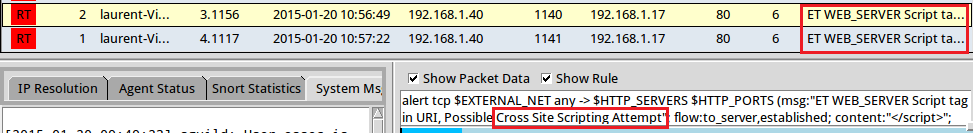
\includegraphics[width=0.85\textwidth]{VM_XSS_5.png}
    \caption{Fortunately, Snort detects the XSS attack without the need for adding additional rules.}
\end{figure}

\begin{figure}[h]
    \centering
    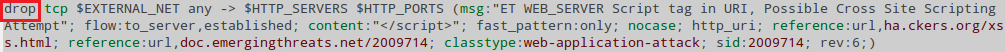
\includegraphics[width=0.85\textwidth]{VM_XSS_6.png}
    \caption{To prevent XSS attacks from happening, one can change ``alert'' to ``drop'' in the rules that triggers the alert.}
\end{figure}

\clearpage

\subsubsection{SQL Injection}

SQL Injection is an attack technique in which users can insert SQL commands as strings that are passed to an SQL server, via a webpage input \citep{SQLInj}. It can be used to read sensitive data from a database or to perform administrative tasks to the database, for example: shutting down the DBMS. \\ \\
To detect such attacks, a custom PHP webpage has been created that is vulnerable to an SQL injection attack. \\ \\
To provide the reader a general overview, the entire content of the MySQL ``Persons'' table is displayed on the webpage. Obviously, in reality, nothing is displayed when a user first loads the page. But the content is displayed for information purposes.
\begin{figure}[h]
    \centering
    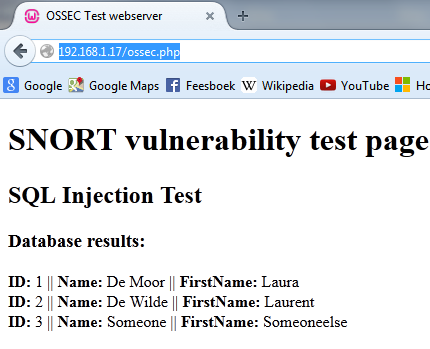
\includegraphics[width=0.85\textwidth]{VM_SQL_1.png}
    \caption{Persons table in the test database running on MySQL 5.6 populated with 3 records.}
\end{figure}
\clearpage
Then, an input textfield is created where the user can enter the firstname of a person he is looking for. The source code is listed below:
\begin{figure}[h]
    \centering
    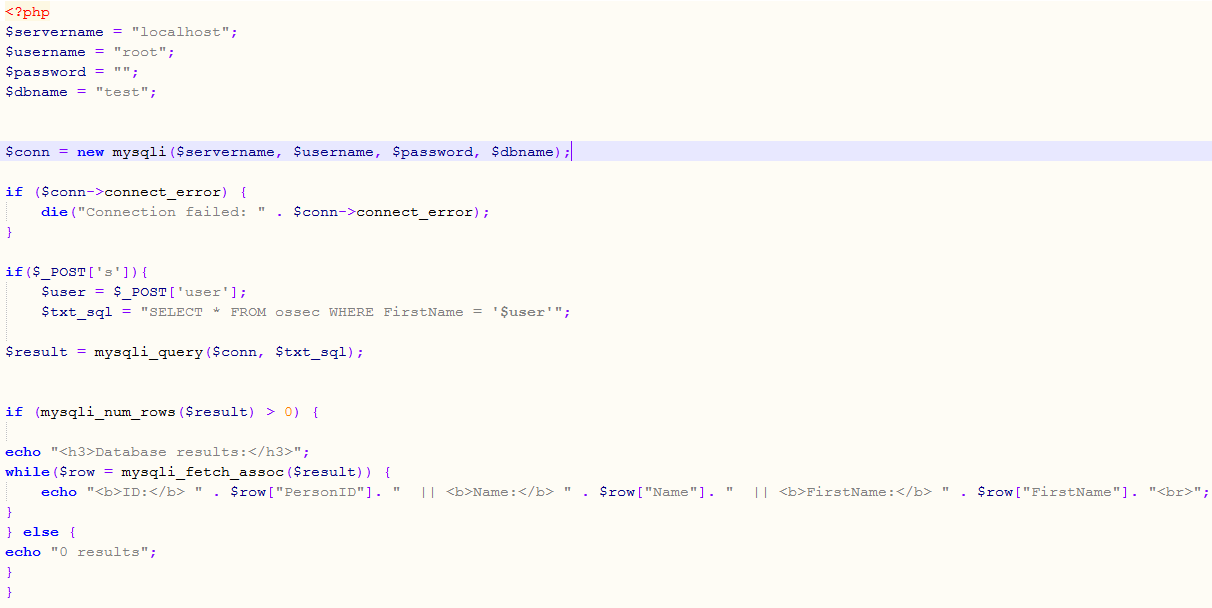
\includegraphics[width=0.85\textwidth]{VM_SQL_3.png}
    \caption{Persons table in the test database running on MySQL 5.6 populated with 3 records.}
\end{figure}
The next screenshot shows an example of how a POST request can look like. In this example, the user has entered the search string ``Laurent".
\begin{figure}[h]
    \centering
    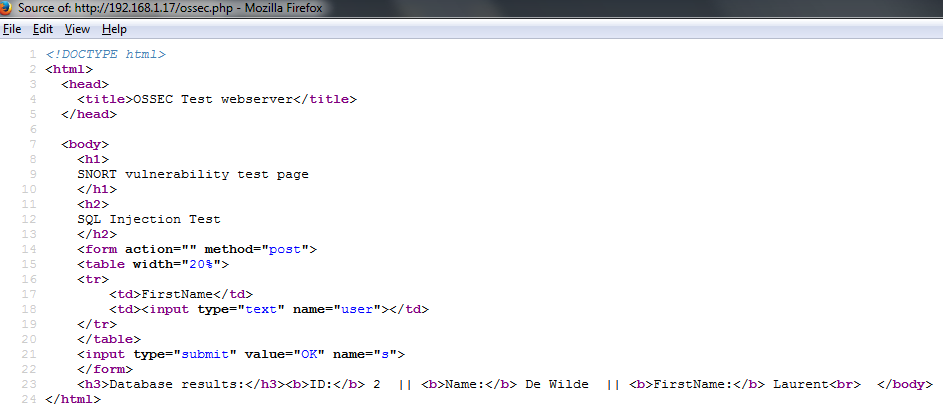
\includegraphics[width=0.85\textwidth]{VM_SQL_2.png}
    \caption{Persons table in the test database running on MySQL 5.6 populated with 3 records.}
\end{figure}
Of course, when the textfield is empty and the query is submitted, nothing is displayed. But when an attacker enters the string ``OR $1=1$'', he gets to see all the information stored in the Persons table. This is called SQL injection based on $1=1$ is always true. It is an attempt to make a query succeed no matter what.
\begin{figure}[h]
    \centering
    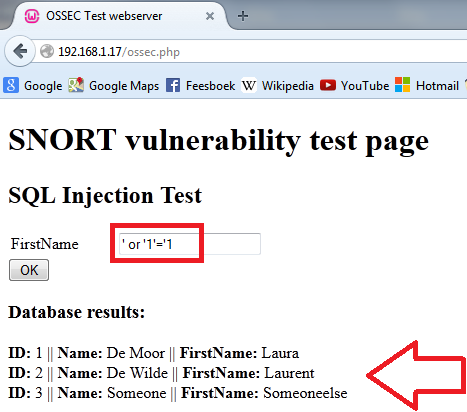
\includegraphics[width=0.85\textwidth]{VM_SQL_4.png}
    \caption{SQL injection attack in action with all the results displayed on the webpage.}
\end{figure}
And did Snort react on this type of webserver attack? Yes it did, as can be seen in the following screenshots:
\begin{figure}[h]
    \centering
    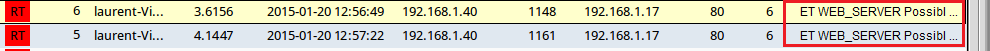
\includegraphics[width=0.85\textwidth]{VM_SQL_8.png}
    \caption{Snort alerts for a possible SQL injection.}
\end{figure}
\begin{figure}[h]
    \centering
    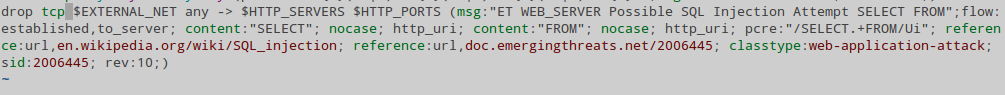
\includegraphics[width=0.85\textwidth]{VM_SQL_9.png}
    \caption{The triggering rule. Once again, one could change ``alert'' to ``drop'' in order to prevent the SQL injection from happening.}
\end{figure}

\clearpage

\subsubsection{Command injection}

A command injection attack is an attack in which a hacker tries to execute commands on the host operating system using a vulnerable (web)application. \\ \\
To simulate this attack, I created a vulnerable PHP webpage that returns the content of a file that the user requested. It does this by executing the ``type'' command on the host machine. But as one may have guessed, an attacker can also execute a command this way.  \\ \\
Following screenshot displays the source code of the webpage.
\begin{figure}[h]
    \centering
    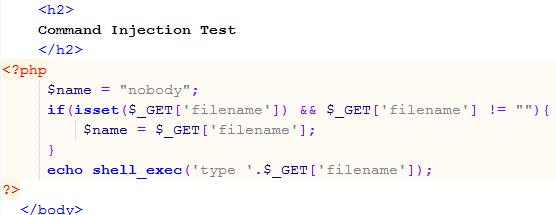
\includegraphics{VM_Command_2.png}
    \caption{The source code of the webpage. Note the ``shell\_exec'' statement. \\}
\end{figure}

An actual example of command injection is listed below. Here, the ``ipconfig'' command is executed on the target host and all information about the network interfaces is returned.
\begin{figure}[h]
    \centering
    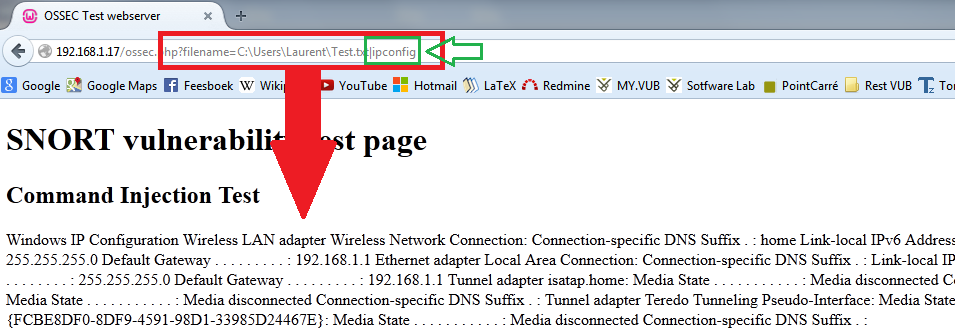
\includegraphics[width=0.95\textwidth]{VM_Command_1.png}
    \caption{An command injection attack has just been launched and the results of executing the ipconfig command are displayed on the webpage.}
\end{figure}
\clearpage
How did Snort react on this thread? Well, at first, i did NOT. Meaning that there are some extra rules needed.
Especially, we want to look for executable files that are passed in the URL, because an attackers usually wants to execute programs (commands) on the host machine. However, it turned out that Snort actually already had a rule that alerts for this kind of attack, but it turned out this rule had been disabled. So enabling the rule was sufficient to make Snort alert on command injection attacks.
\begin{figure}[h]
    \centering
    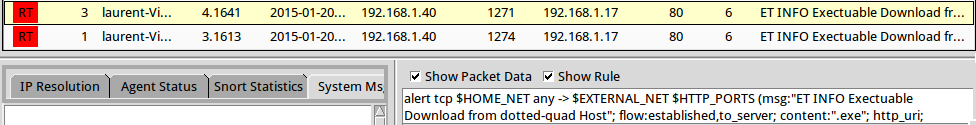
\includegraphics[width=0.95\textwidth]{VM_Command_3.png}
    \caption{Snort alerting for command injections}
\end{figure}

\clearpage

\subsection{FTP server attacks}

To test for attacks on FTP servers running on the network, I have set up an FTP server with FileZilla Server 0.9.49. On the attacking machine, all FTP attacks were launched from FileZilla Client 3.10.

\subsubsection{Testing for FTP Traffic}

In order to make sure that FTP is actually picked up by Snort (that is, all traffic to port 21), a simple rule has been set up to do so.
\begin{figure}[h]
    \centering
    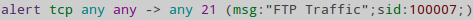
\includegraphics{VM_FTP_2_1.png}
    \caption{Rule for alerting on any traffic on port 21}
\end{figure}
Which yields following output when connecting to the FTP server:
\begin{figure}[h]
    \centering
    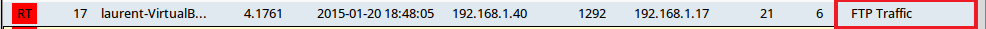
\includegraphics[width=0.95\textwidth]{VM_FTP_4_1.png}
    \caption{OK!}
\end{figure}

\subsubsection{FTP Root access}

Now that we are sure that FTP traffic gets picked up by Snort, we can begin to detect root access. If an attacker is able to login as root, he gains full control over the target host. Let us first check if Snort is able to detect root login out of the box.
\begin{figure}[h]
    \centering
    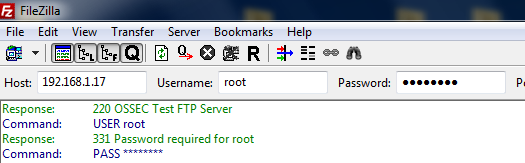
\includegraphics[width=0.95\textwidth]{VM_FTP_3.png}
    \caption{Logging in as root\ldots}
\end{figure}
As it turns out, Snort did NOT pick up any root login attempts. Thus extra rules have to be added to extends Snort's functionality. This is shown in the following screenshot.

\clearpage

\begin{figure}[h]
    \centering
    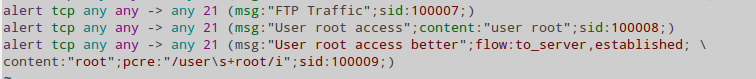
\includegraphics[width=0.95\textwidth]{VM_FTP_2.png}
    \caption{Additional rules for detecting root logins.}
\end{figure}
When the rules are added, Snort is restarted and root login is performed again. This time, Snort was able to detect root login on the FTP server.
\begin{figure}[h]
    \centering
    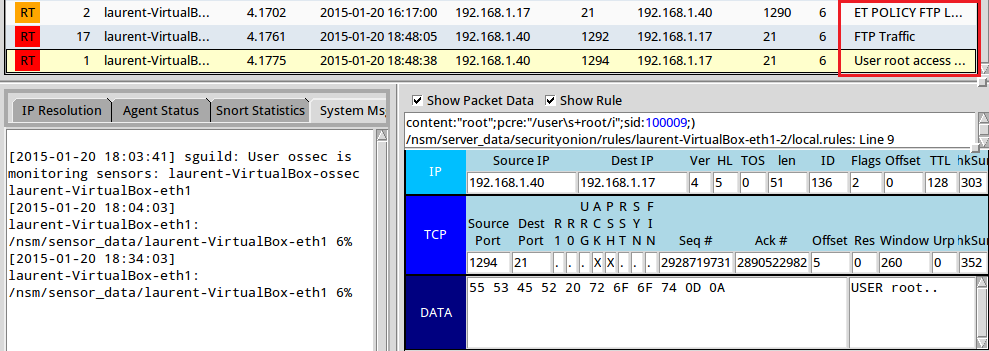
\includegraphics[width=0.95\textwidth]{VM_FTP_4.png}
    \caption{This time, Snort detects root logins. Note that this can be prevented by changing ``alert'' to ``drop''.}
\end{figure}

\subsubsection{FTP attack using Metasploit}

There exist some rules that the Snort community has created for us that protects our FTP server even better. Let us download these rules and activate them. The file is called ``ftp.rules'' and can be found online.

First, one has to include the file in ``snort.conf'':
\begin{figure}[h]
    \centering
    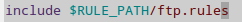
\includegraphics{VM_FTP_5.png}
    \caption{Include the downloaded rules in Snort.}
\end{figure}

Now that we have the availability of quite powerful FTP anomaly detection, it is time to perform some `FTP bashing'. We will use Metasploit for this purpose.

Metasploit is a penetration testing program capable of performing various types of attacks. We will use the ``db\_autopwn'' module of Metasploit.

\begin{figure}[h]
    \centering
    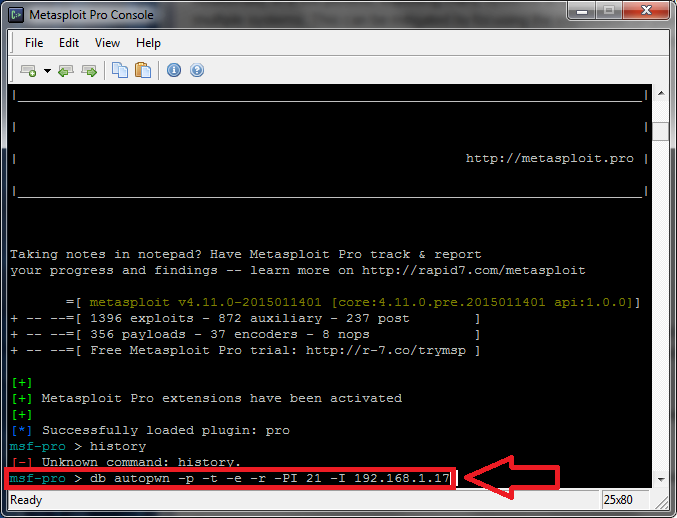
\includegraphics[width=0.95\textwidth]{VM_FTP_8.png}
    \caption{Ready to perform the pownage on port 21 of the victim with IP address of 192.168.1.17}
\end{figure}
After the pownage has completed, we look into Sguil to find following alerts:
\begin{figure}[h]
    \centering
    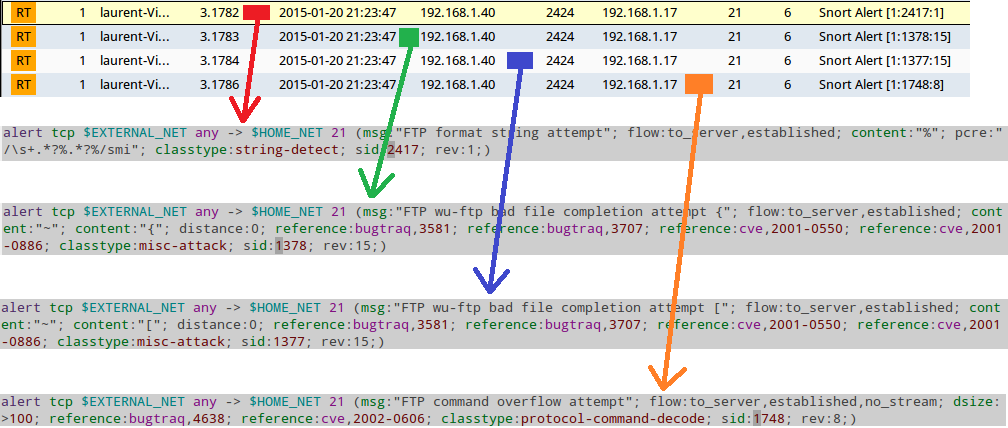
\includegraphics[width=0.95\textwidth]{VM_FTP_7.png}
    \caption{Snort is able to catch the attacks peformed on the FTP server.}
\end{figure}
As is turns out, Snort has captured various types of attack that Metasploit performed on the FTP server. Note that all these alerts are generated by the rules in the ftp.rules file that we downloaded. Thus, without those rules, nothing would have been captured.

\clearpage

\subsection{SSH attacks}

In this section, we will focus on bruteforcing (dictionary attacking) an SSH server using a file that contains the usernames and another file containing the passwords that the bruteforce (dictionary attack) will use to try logging in into the SSH server (and thus getting access to the host).

\subsubsection{SSH bruteforcing}

Again, we will make use of Metasploit to perform the SSH bruteforce attack. This time, the ``ssh\_login'' module will be used.

\begin{figure}[h]
    \centering
    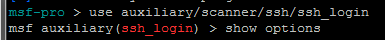
\includegraphics{VM_SSH_3.png}
    \caption{The required SSH login plugin is loaded into Metasploit}
\end{figure}

The module is configured for the bruteforce attack: the RHOST (remote host) is set, the file containing the username and passwors is set, as well as verbose mode.

\begin{figure}[h]
    \centering
    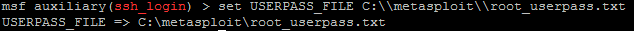
\includegraphics[width=0.95\textwidth]{VM_SSH_4.png}
    \caption{The file containing the usernames and passwords is loaded into Metasploit.}
\end{figure}

\begin{figure}[h]
    \centering
    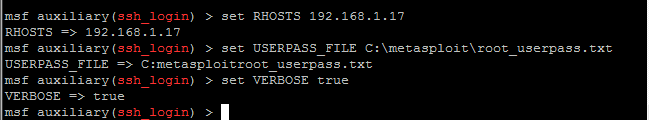
\includegraphics[width=0.95\textwidth]{VM_SSH_2.png}
    \caption{Some other options are configured and everything is put together.}
\end{figure}
Eventually, the actual bruteforcing attack is started and one can observe that every entry in the file is read, tested against (on) the SSH server and in case of failure, the next line is read.

However, in case of a successful username/password combination, the attack is stopped and the username:password is displayed. Now the attacker (us) has the ability to login into the system and he can perform some malicious operations.
\begin{figure}[h]
    \centering
    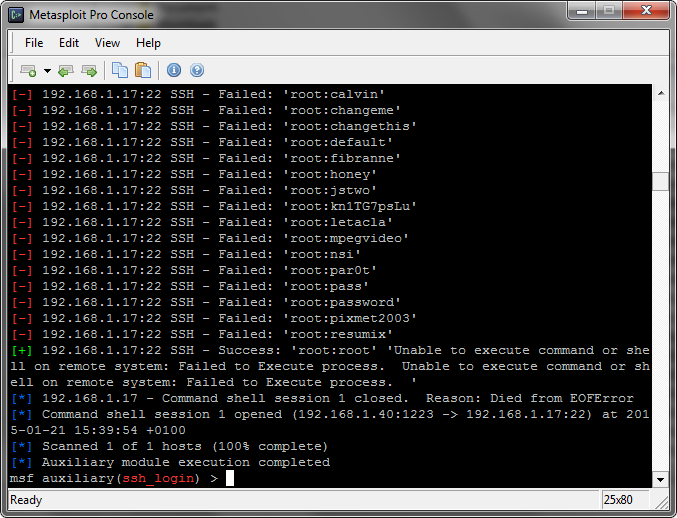
\includegraphics[width=0.95\textwidth]{VM_SSH_5.png}
    \caption{Bruteforcing in action\ldots}
\end{figure}
But what about Snort? Did Snort detect the bruteforce attempt? The answer is YES. It actually detects SSH bruteforcing out of the box. So, no additional rules need to be added.

\begin{figure}[h]
    \centering
    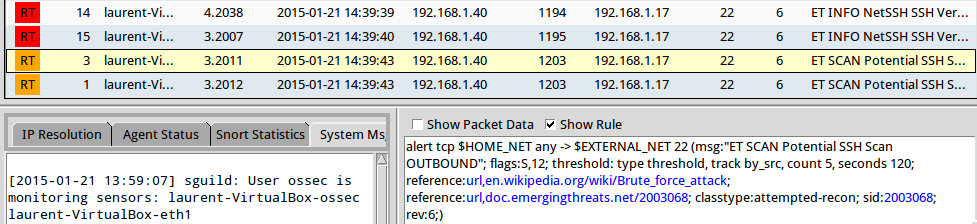
\includegraphics[width=0.95\textwidth]{VM_SSH_6.png}
    \caption{Snort alerting for SSH bruteforcing.}
\end{figure}

\clearpage

\subsection{SMB attacks}

When an attacker performs a port scan and notices that port 139 and 445 are open, he knows that a Sambda (file sharing) server is running on the host. Then he can perform some attacks on the SMB (Samba) server including bruteforce logins, enumerating the shares, \ldots.

We will again use Metasploit to perform some attacks on our file server.

\subsubsection{Bruteforcing (dictionary attacking) an SMB server}

Bruteforcing the SMB server will be performed by a seperate username file and a password file. The password file is retrieved from ``John-The-Ripper'', a password cracker. Remains the file with the usernames. 

However, nowadays there exist a vast amount of social networking websites so why don't we retrieve a list of usernames from one of those social networking sites? Since Facebook is the most popular social networking site in Belgium \citep{Facebook}, we tried and succeeded in retrieving a file that contains (nearly) all the firstnames of the Facebook users as of 2010.

Both files are loaded into Metasploit. The ``smb\_login'' module is used to bruteforce the server. Every combination of a username and password listed in these files will be tried. 
\begin{figure}[h]
    \centering
    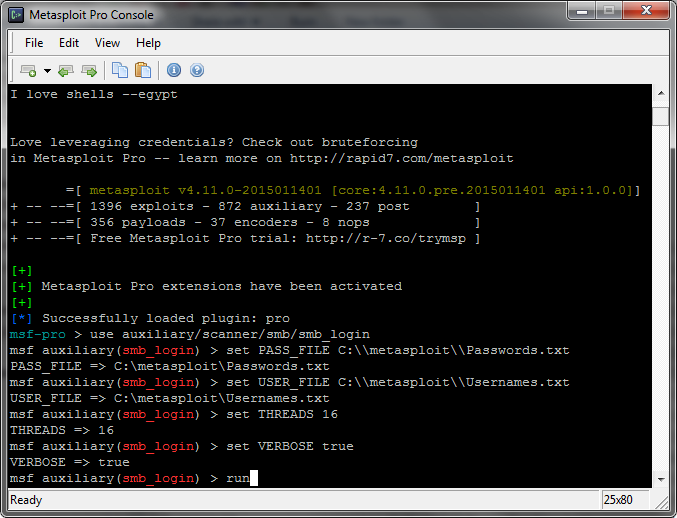
\includegraphics[width=0.95\textwidth]{VM_SMB_5.png}
    \caption{Bruteforce the Samba server using a seperate username and password file.}
\end{figure}

\clearpage
So did Snort detect those login attempts? YES, it did, as can be seen in the following screenshot. This means that no rules have to be added.
\begin{figure}[h]
    \centering
    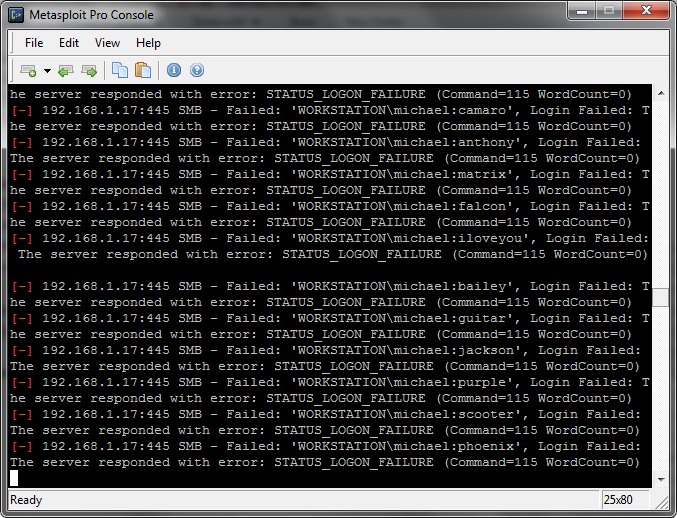
\includegraphics[width=0.95\textwidth]{VM_SMB_6.png}
    \caption{Bruteforce process in action\ldots}
\end{figure}

\begin{figure}[h]
    \centering
    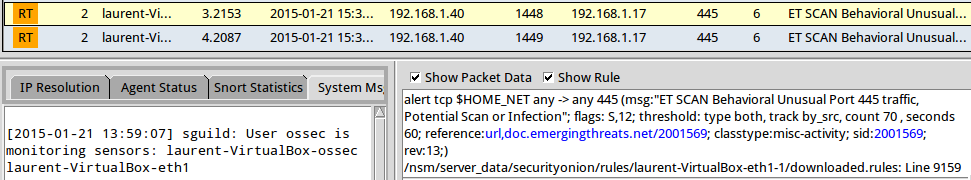
\includegraphics[width=0.95\textwidth]{VM_SMB_9_scan.png}
    \caption{Snort detects the bruteforcing attempts and alerts so.}
\end{figure}

\begin{figure}[h]
    \centering
    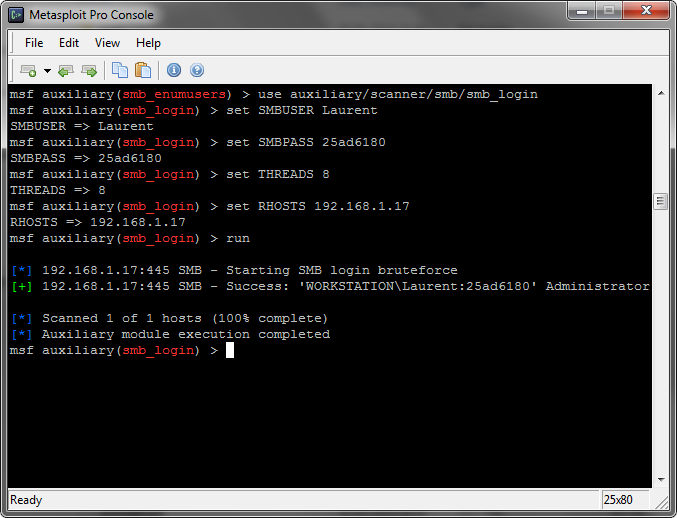
\includegraphics[width=0.95\textwidth]{VM_SMB_4.png}
    \caption{Confirmation that one is able to login with the credentials found by the bruteforcing attack.}
\end{figure}

\clearpage

\subsubsection{List the shares on an SMB server}

Once the attacker knows a valid username:password combination, he can begin querying the system. For example, he could list the available shares on the system, as well as listing the registered users on the target system.

\begin{figure}[h]
    \centering
    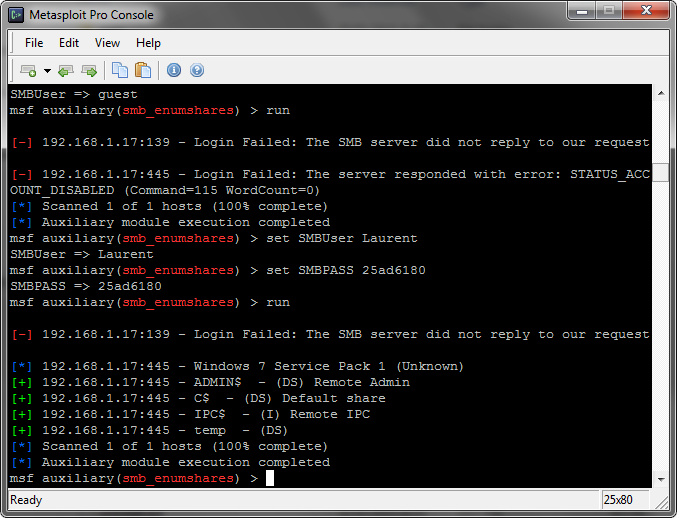
\includegraphics[width=0.95\textwidth]{VM_SMB_2.png}
    \caption{Listing of the available shares on the target server.}
\end{figure}

\begin{figure}[h]
    \centering
    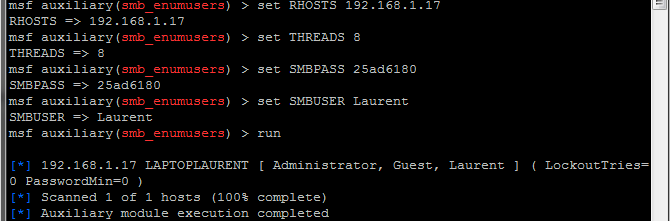
\includegraphics[width=0.95\textwidth]{VM_SMB_3.png}
    \caption{Listing of the available users on the target server.}
\end{figure}

But how did Snort react on those malicious login attempts? Well, since listing the shares and the users requires shares access, Snort did alert that share access had taken place. In addition, it turned out that the username:password found by the bruteforcing attacks was an administrator account. Snort made the distinction between regular share access or share access performed by an admin account.

\begin{figure}[h]
    \centering
    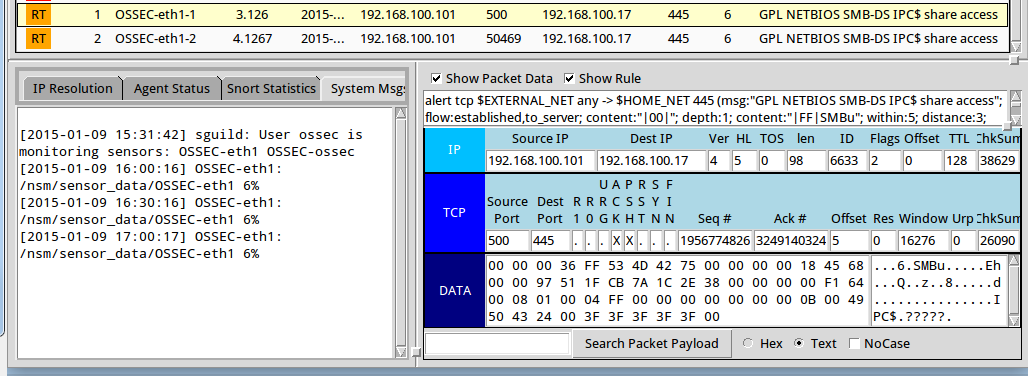
\includegraphics[width=0.95\textwidth]{VM_Share.png}
    \caption{Detecting regular share access\ldots}
\end{figure}

\begin{figure}[h]
    \centering
    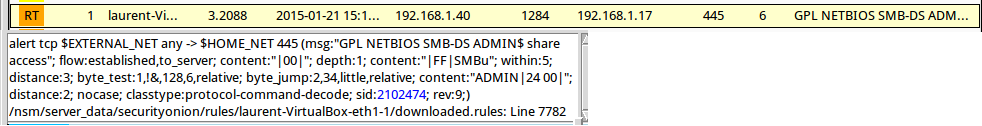
\includegraphics[width=0.95\textwidth]{VM_SMB_8_admin_share_access.png}
    \caption{and detecting admin share access.}
\end{figure}

Of course, Snort cannot know that we retrieved those credentials in a malicious way. \\ \\

So the actual process of listing the shares was NOT detected. Unfortunately, no specific rules exist, nor was I able to write rules that alerts for listing shares. Obviously, one can write a rule that alerts for ALL traffic on port 139 or 445, but this would be a very noisy rule and we want to avoid this.

\clearpage

\subsection{Database attacks}

In this section, we will investigate how well Snort alerts for database attacks and determine if extra configuration is needed. The database running on the test server is MySQL 5.6.

\subsubsection{Database scanning}

In a first step, we want to check which hosts on the network are running MySQL servers. So let us scan a part of the network for open 3306 (MySQL) ports.

\begin{figure}[h]
    \centering
    \includegraphics[width=0.95\textwidth]{VM_MSSQL_2.png}
    \caption{Looking for MySQL servers running on the network\ldots}
\end{figure}

Did Snort see this malicious activity? YES, it did! No further configuration is needed.
\begin{figure}[h]
    \centering
    \includegraphics[width=0.95\textwidth]{VM_MSSQL_3.png}
    \caption{Snort does not agree with this and sends an alert}
\end{figure}

So Snort detects MySQL scans out-of-the-box. But maybe we can add some additional rules to provide us with some more detailed information? For example, we are interested if someone (an attacker) tries to login as root or tries to list the databases available on the MySQL server.
\begin{figure}[h]
    \centering
    \includegraphics[width=0.95\textwidth]{VM_MSSQL_5.png}
    \caption{Additional rules for detecting root login and showing databases.}
\end{figure}

Let us perform these two steps at once:

\begin{figure}[h]
    \centering
    \includegraphics[width=0.95\textwidth]{VM_MSSQL_4.png}
    \caption{The attacker logs in as root and wants to see all the databases\ldots}
\end{figure}

Did our additional rules work? I.e., did Snort alert for this two actions? Yes, it did!

\begin{figure}[h]
    \centering
    \includegraphics[width=0.95\textwidth]{VM_MSSQL_6.png}
    \caption{The added rules work!}
\end{figure}

\clearpage

\subsubsection{Database login bruteforcing}

Now that an attacker (us) knows which servers are running MySQL databases, he could perform a bruteforce attack on that server in order to be able to login into the system and manipulate the databases.

\begin{figure}[h]
    \centering
    \includegraphics[width=0.95\textwidth]{VM_MSSQL_7.png}
    \caption{Bruteforce attack in action\ldots}
\end{figure}
How did Snort react on our bruteforce attack? Well, it detected suspicious activity and generated corresponding alerts. No further configuration is needed. Of course, one could change to rule so that Snort does not alert, but rather drops (and therefore prevents) the attack. This can be achieved by changing ``alert'' to ``drop''.
\begin{figure}[h]
    \centering
    \includegraphics[width=0.95\textwidth]{VM_MSSQL_8.png}
    \caption{The bruteforce attack is reported.}
\end{figure}

\clearpage

\subsection{Trojan injections}

Let us try some more serious stuff, for example inserting / injecting a trojan on a target host. A trojan for a Windows machine will be created and make it connect to us.

A trojan is a program in which malicious and harmful code is encapsulated by apparently harmless code. \\ \\
We will use Metasploit once again to generate such a trojan. How will this be achieved? We will use a Metasploit module called ``msfpayload'' to generate a file that contains malicious code. We choose the payload we want to use. In this case we use reverse TCP. This is a way to get around the firewall.

We set the LHOST (local host), so that the trojan will connect to our computer, the port number and the filename of the file that will be generated. In real life, one would email this program to the victim, but for this testing purposes, we just place in on the desktop of the victim. 

\begin{figure}[h]
    \centering
    \includegraphics[width=0.95\textwidth]{VM_Trojan_2.png}
    \caption{Setting up the trojan.}
\end{figure}
As one can see, the file is generated and placed on our desktop.
\begin{figure}[h]
    \centering
    \includegraphics{VM_Trojan_6.png}
    \caption{The generated trojan horse.}
\end{figure}
Then we are going to make a listener that actually waits for the trojan to be executed on the target host. 
\begin{figure}[h]
    \centering
    \includegraphics[width=0.95\textwidth]{VM_Trojan_3.png}
    \caption{Setting up the listener.}
\end{figure}

\begin{figure}[h]
    \centering
    \includegraphics[width=0.95\textwidth]{VM_Trojan_5.png}
    \caption{A user has clicked on the trojan and a sessions has been opened.}
\end{figure}

\clearpage

When the session is established, we have remote access to the victim's machine. We can for example view the network configuration of the remote host or list the directory structure of it's C: drive.
\begin{figure}[h]
    \centering
    \includegraphics[width=0.95\textwidth]{VM_Trojan_4.png}
    \caption{Executing some commands on the victim\ldots}
\end{figure}
What was the reaction of Snort to this attack? It reported some suspicious activity and corresponding alerts were generated. No further configuration is required.
\begin{figure}[h]
    \centering
    \includegraphics[width=0.95\textwidth]{VM_Trojan_1.png}
    \caption{The attack is reported.}
\end{figure}

\clearpage

\subsection{DOS attacks}

The final attack discussed is a denial-of-service (DOS) attack performed on the victim host. We make use of a specialized program called `Low Orbit Ion Cannon' for this purpose. We will perform an HTTP DOS attack on our webserver that we previously set up for simulating XSS attacks and SQL injections. \\ \\
The address of the webserver is filled in, as well as the number of threads and the port number. Next, the attack is performed.

\begin{figure}[h]
    \centering
    \includegraphics[width=0.95\textwidth]{VM_DOS_1.png}
    \caption{Initiating the attack.}
\end{figure}

\begin{figure}[h]
    \centering
    \includegraphics[width=0.45\textwidth]{VM_DOS_3.png}
    \caption{The DOS attack in action as seen from Windows Task Manager.}
\end{figure}
\clearpage
\begin{figure}[h]
    \centering
    \includegraphics[width=0.85\textwidth]{VM_DOS_4.png}
    \caption{The DOS attack in action as seen in Wireshark.}
\end{figure}
Fortunately, Snort did detect the attack and corresponding alerts were raised. This means that no further action is required. Of course, one can also block these attacks by, instead of alerting, dropping the packets.
\begin{figure}[h]
    \centering
    \includegraphics[width=0.95\textwidth]{VM_DOS_2.png}
    \caption{The attack is reported by Snort.}
\end{figure}

\clearpage

\section{False alerts}

On all the physical machines, Dropbox is installed. Apperantly, Dropbox sends broadcasting messages from time to time. According to Dropbox, this is caused by a feature called ``Lan sync''. When a user adds or modifies a file in the Dropbox folder, it is first synced with the computers that are running the Dropbox client on the same subnet. After this, the changes are uploaded to the Dropbox servers \citep{Dropbox}. \\ \\
This is an example of a false alert and one wants to prevent this alert from raising more messages. Therefore, one can comment the rule that is causing the alerts, as is illustrated in the following screenshot.

\begin{figure}[h]
    \centering
    \includegraphics[width=0.95\textwidth]{VM_Dropbox.png}
    \caption{Snort sees the broadcasting of Dropbox as an intrusion. This can be fixed by commenting the rule that is triggering the alert.}
\end{figure}

\clearpage

\section{Additional configuration and fine-tuning Sguil}

Now that we have a huge amount of alerts at our disposal, it is time to clean things up. When suspicious activity is detected, Sguil classifies those alerts as realtime (RT) events and puts them all in one single overview.

However, after some time of testing, this overview table can quickly fill up with hundreds of alerts. Fortunately, Sguil offers the possibilty to classify alerst into different categories. Those categories are:
\begin{enumerate}
\item F1: Category I: Unauthorized Root/Admin access.
\item F2: Category II: Unauthorized User access.
\item F3: Category III: Attempted Unauthorized Access
\item F4: Category IV: Successful Denial-of-Service Attack
\item F5: Category V: Poor Security Practice or Policy Violation
\item F6: Category VI: Reconnaissance/Probes/Scans
\item F7: Category VII: Virus Infection
\item F8: No action necessary
\end{enumerate}

By clicking a RT (realtime) event and pressing the corresponding function (Fx) key, the alert is moved to the designated category. This process is called manual classification of events. \\ \\
Following screenshots show the different categories applied at our situation:

\begin{figure}[h]
    \centering
    \includegraphics[width=0.95\textwidth]{VM_CAT_3.png}
    \caption{Category II (C2): FTP Root access falls into this category.}
\end{figure}

\begin{figure}[h]
    \centering
    \includegraphics[width=0.95\textwidth]{VM_CAT_5.png}
    \caption{Category III (C3): MySQL bruteforcing falls into this category.}
\end{figure}
\clearpage
\begin{figure}[h]
    \centering
    \includegraphics[width=0.95\textwidth]{VM_CAT_4.png}
    \caption{Category IV (C4): the DOS attack on our webserver can be put in this category.}
\end{figure}

\begin{figure}[h]
    \centering
    \includegraphics[width=0.95\textwidth]{VM_CAT_1.png}
    \caption{Category VI (C6): Portscans can be placed in this category.}
\end{figure}

\begin{figure}[h]
    \centering
    \includegraphics[width=0.95\textwidth]{VM_CAT_2.png}
    \caption{Category VII (C7): The trojan falls into this category.}
\end{figure}
\clearpage
\begin{figure}[h]
    \centering
    \includegraphics[width=0.95\textwidth]{VM_CAT_6.png}
    \caption{Non classified: ICMP ping traffic.}
\end{figure}

However, this process can be automated. Therefore, one has to adjust the file ``autocat.conf''. Some rules have been written for our network in order to automatically classify certain events.

\begin{figure}[h]
    \centering
    \includegraphics[width=0.95\textwidth]{VM_CAT_7.png}
    \caption{Custom rules added to the file ``autocat.conf''. For example, VISA transferred in plain text over the network is automatically placed in category V (5).}
\end{figure}

\clearpage

\subsection{Configuring Sguil}

As previously mentionend, the generated Sguil alerts are stored in a MySQL database. We can gain access to this database in order to execute some queries to further investigate which rules need additional configuration. Some overly active rules can be surpressed and thresholds can be set as well. \\ \\
Below is a part of the tables in the Sguil database.

\begin{figure}[h]
    \centering
    \includegraphics[width=0.55\textwidth]{VM_DB_1.png}
    \caption{107 tables are present in the Sguil database at the time of capturing this screenshot. Note that per day, additional tables are added.}
\end{figure}
\clearpage
All alerts are stored in the ``event'' table. Let us find out how many events that have been generated after the testing period.

\begin{figure}[h]
    \centering
    \includegraphics{VM_DB_2.png}
    \caption{271307 events were generated IN TOTAL.}
\end{figure}

\subsubsection{Listing the top 20 signatures}

Listing the top 20 signatures can be handy as this allows us to fine-tune the rule that is causing so many alerts. Not only does a huge amount of alerts slow down Sguil, it will cost the user time that could better be used to focus on alerts with greater significance.

\begin{figure}[h]
    \centering
    \includegraphics[width=0.95\textwidth]{VM_DB_4.png}
    \caption{One can observe that the rule `HTTP Traffic' has been triggered many times.}
\end{figure}
It can be useful to list the IP addresses from the computers that generated the alert. Of course, since in our test lab, we only have one attacking machine, only one IP address will be listed.
\begin{figure}[h]
    \centering
    \includegraphics[width=0.95\textwidth]{VM_DB_4.png}
    \caption{The HTTP alerts came from a host with IP address 192.168.1.40.}
\end{figure}

\subsubsection{Setting thresholds and limitations on alerts}

In order to temper the activity of some rules, one can set thresholds and suppressions on them. \\ \\
The general format of suppressing a rule is as follows: \\
\textbf{suppress gen\_id gen-id, sig\_id sid-id, track [by\_src|by\_dst], ip IP/MASK-BITS} \\ \\
The general format of event\_filter a rule is as follows: \\


But in order to do so, we first have to know the generator ID. (This mostly will be 1).

\begin{figure}[h]
    \centering
    \includegraphics[width=0.95\textwidth]{VM_DB_7.png}
    \caption{The HTTP alerts came from a host with IP address 192.168.1.40.}
\end{figure}

Then, the process of setting up thresholds and limitations can begin as is shown in following screenshots.

\begin{figure}[h]
    \centering
    \includegraphics[width=0.95\textwidth]{VM_DB_8.png}
    \caption{Limitation: here we limit the alerting of signature `HTTP Traffic' to 100 every hour.}
\end{figure}

\begin{figure}[h]
    \centering
    \includegraphics[width=0.95\textwidth]{VM_DB_9.png}
    \caption{Combination of suppression and limitation: alert every 1 time the `HTTP Traffic' rule is triggered during a half-hour interval.}
\end{figure}

\begin{figure}[h]
    \centering
    \includegraphics[width=0.95\textwidth]{VM_DB_10.png}
    \caption{Suppression: here we suppress `HTTP Traffic' completely for the host with IP address 192.168.1.40 (the host were the alerts originated.}
\end{figure}











